\capitulo{5}{Aspectos relevantes del desarrollo del proyecto}

    Antes de hablar y profundizar sobre EDVR, el modelo implementado en el Trabajo de fin de grado, se explicará el concurso del que fue ganador en las categorías de vídeo, NTIRE Challenge 2019.
    
    \section{NTIRE Challenge video 2019}

   NTIRE (New Trends in Image Restoration and Enhancement) challenge es un workshop que lleva realizándose desde 2017. El objetivo que ha tenido y tiene siempre es presentar los avances y tendencias en el campo de la restauración y mejora de imágenes y vídeos. También pretende servir como punto de encuentro entre empresas y desarrolladores para lograr colaboraciones. 

    Siempre distingue entre dos tipos generales de retos, que son problemas expuestos por los organizadores que plantean dificultades de ejecución, y cada uno de estos retos se divide a su vez en otros más especializados.
    \begin{itemize}
    \item Retos de imágenes
    \item Retos de vídeos
    \end{itemize}
    
    Por la naturaleza del trabajo solo nos centraremos en los retos del 2019 en la categoría de vídeos, los cuales fueron ganados por EDVR.
    
    \subsection {Challenge on video Super-Resolution ~\cite{Nah_2019_CVPR_Workshops}}
        Los objetivos de este reto son: impulsar las técnicas actuales de super resolución, comparar diferentes soluciones, promover el uso del dataset REDS y promover retos más difíciles para la super resolución de vídeos.
        
        \begin{itemize}
        \item\textbf {\emph{Track 1 clean}} Versión adaptada para métodos comunes de super resolución, ya que emplea degradación mediante submuestreo bicúbico de factor 4, las imágenes tienen un tamaño 4 veces menor al original.
        
        \item\textbf {\emph{Track 2 blur }} Versión más complicada, ya que incluye emborronamientos debido a objetos en movimiento y a movimiento de cámaras.  Son vídeos más acordes con la realidad.
        \end{itemize}
        
    \subsection {Challenge on video Deblurring ~\cite{NITRE_CVD}}
        Los objetivos de este reto son: impulsar las técnicas actuales de eliminación de emborronamiento, comparar diferentes soluciones, promover el uso del dataset REDS y promover retos más difíciles para el desemborronamiento de vídeos.  

        \begin{itemize}
        \item\textbf {Track 1 clean} Versión adaptada para métodos comunes para la eliminación de emborronamientos de vídeos. Los emborronamientos son los propios del movimiento de la cámara y de los objetos en movimiento.
        
        \item\textbf {Track 2 compression artifacts} Se incluye los mismos problemas que el apartado anterior pero ahora los vídeos presentan compresión del 60\%.
        \end{itemize}

\section{REDS}
    REalistic and Dynamic Scenes~\cite{Nah_2019_CVPR_Workshops_REDS}, es el dataset oficial del NITRE Challenge vídeo y aspira a ser un referente en el aparatado de la super resolución y desemborronamiento de vídeos.
    
    Compuesto por 30.000 imágenes extraídas de vídeos grabados por el equipo que lo desarrolla. La resolución se asemeja a los estándares actuales siendo de $720\times 1280$. La manera de crear las imágenes borrosas naturales consiste en aumentar los fotogramas por segundo (fps), y usar una red neuronal convolucional (CNN) para rellenar los detalles perdidos.
    
    El dataset está dividido en 5 apartados:
        \begin{itemize}
        \item\textbf {Original} También conocido como GT (Ground Truth). Se usan principalmente como imágenes de referencia con que comparar  las imágenes obtenidas por los métodos de super resolución/restauración.
        \item\textbf {Borroso.} 
        \item\textbf {Borroso y comprimido.} 
        \item\textbf {Baja resolución.} 
        \item\textbf {Borroso y baja resolución.} 
        \end{itemize}
    El dataset puede ser descargado aquí: \url{https://seungjunnah.github.io/Datasets/reds.html}

\section{Vimeo 90K}
    Es un dataset desarrollado mediante la selección de vídeos de la plataforma Vimeo para un modelo de mejora de vídeos basado en la estimación de los movimientos~\cite{xue2019video}. Una red neuronal con un componente de entrenamiento  para la predicción de movimiento y el procesamiento de vídeo.
    
    Formado por casi 90.000 clips de vídeos con multitud de escenarios y diversidad. Creado específicamente para la restauración de vídeos. Todos los clips tienen un tamaño estándar de $448\times 256$ píxeles.
    
    El dataset puede ser descargado aquí: \url{http://toflow.csail.mit.edu/}
    
\section{Estructura y funcionamiento de EDVR}    

    EDVR ~\cite{wang2019edvr} es el acrónimo de Enhanced Deformable convolutions Video Restoration, es una herramienta contenida en BasicSR (\emph{Basic Super Restoration}), un proyecto OpenSource de restauración para imágenes y vídeos, que también contiene a EDSR (\emph{Enhanced Deep Residual Networks}), RCAN (\emph{Residual Channel Attention Networks}), SRResNet (\emph{Super Resolution ResNet}), SRGAN (\emph{Super Resolution Generative Adversarial Network}), ESRGAN (\emph{Enhanced Super-Resolution Generative Adversarial Networks}), StyleGAN2 (\emph{Style Generative Adversarial Network 2}) y DFDNet (\emph{Dictionary Feature Transfer Net}).
    
    EDVR está basado en dos módulos fundamentales que son los responsables de la eficiencia del método. Un módulo de alineamiento de convoluciones PCD (\emph{Pyramid, Cascading and Deformable}) y un módulo de fusión TSA (\emph{Temporal and Spatial Attention}). Partiendo de $2N+1$ fotogramas en baja calidad, denominamos  $I_t$ al fotograma central  y el resto se denominan fotogramas adyacentes. El objetivo de la restauración de vídeo es estimar una imagen de alta calidad que se asemeje a la imagen de referencia, GT.

    \imagen{frameworkEDVR}{Estructura de funcionamiento interno EDVR~\cite{wang2019edvr}}
    
    Previo a la aplicación de PCD y TSA, se ofrece la posibilidad de aplicar un módulo de  eliminación del emborronado a las imágenes de entrada para mejorar el alineamiento de características.
    
    \subsection {PCD}
        Acrónimo de \emph{Pyramid, Cascading and Deformable convolution} inspirado por TDAN (\emph {Temporally Deformable Alignment Network}) ~\cite{tian2018tdan}, que también usa el alineamiento mediante convoluciones deformables(operaciones de pequeñas agrupaciones de píxeles para puntuar las características de la imagen) para los alinear las características de los fotogramas adyacentes. 

        \imagen{PCD}{Módulo PCD \emph{Pyramid, Cascading and Deformable convolution} de EDVR~\cite{wang2019edvr}}
    
        Partiendo de un núcleo de convolución deformable de $K$ posiciones de muestreo, se denota $w_k$  y  $p_k$ al peso y a las compensaciones preestablecidas para cada posición $K$. Las características alineadas  en cada posición  $p_0$ se obtienen por:
        \begin{equation}\label{12}
            F^a_{t+i} (p_0) = \sum^K_{k=1} w_k * F_{t+1}(p_0 + p_k +\Delta p_k) * \Delta m_k
        \end{equation}
      Donde * es el operador de convolución y la compensación aprendible $\Delta p_k $ y el escalar de modulación $\Delta m_k $ son predichos concatenando características del fotograma central y los adyacentes.
        
         \begin{equation}\label{27}
          \Delta P_{t+i} = f([F_{t+i}, F_t]), i \in [-N:+N]
        \end{equation}
        
        \noindent $f$ es una función general de varias capas de convolución y  [·, ·] es la concatenación.
        La principal diferencia es el modo de hacerlo, se usa una estructura piramidal que primero se centra en la alineación de las características de los detalles de manera amplia, para luego aumentar la perspectiva y compensar de manera precisa los movimientos.
        
        Para generar la característica $F^l_{t+i}$ en los niveles se usan filtros de convolución estriados(mayor desplazamiento de las agrupaciones de píxeles) para reducir la muestra de las características en $l-1$ nivel de la pirámide en un factor de 2, obteniendo pirámides de representación de características de $L$ niveles. En los niveles los desplazamientos y el lineamiento de características también son predichas con los desplazamientos x2 y las características del nivel $l+1$.

        \begin{equation}\label{39}
          \Delta P_{t+i} = f([F_{t+i}, F_t], (\Delta P^{l+1}_{t+i})^{\uparrow 2})
          (F^a_{t+1})^l = g(DCon(F^l_{t+i},\Delta P^l_{t+i}), ((F^a_{t+i})^{l+1})^{\uparrow 2})
        \end{equation}

        $(.)^{\uparrow s}$ es el factor de escalado, DConv es la convolución deformable de la primera fórmula y g es  una función general con varias capas de convolución. 
        EDVR usa una pirámide de 3 niveles.
         Adicionalmente se realiza una convolución deformable que mejora la alineación.

    \subsection {TSA}
        Acrónimo de \emph{Temporal and Spatial Attention} ayuda al añadido de información a través de las características alineadas. Para eso se usa la fusión con atención temporal(proceso para centrarse en los aspectos relevantes de una secuencia) para calcular la correlación entre el fotograma central y los adyacentes. Estos cálculos se usan para saber cuáles son las mejores características que se usaran para reconstruir el fotograma central. Tras esto se aplica la atención espacial para asignar pesos a las ubicaciones en cada canal para compartir información entre canales.
        
        \imagen{TSA}{Módulo TSA \emph{Temporal and Spatial Attention} de EDVR~\cite{wang2019edvr}}
    
        Para cada fotograma la distancia de similitud $h$ se calcula con:
        \begin{equation}\label{48}
        \tilde{F}^a_{t+i} = F^a_{t+i} \odot h(F^a_{t+i}, F^a_t)
        F_{fusion} = Conv(\tilde{F}^a_{t-N}, \cdot\cdot\cdot, \tilde{F}^a_{t},\cdot\cdot\cdot, \tilde{F}^a_{t+N} )
        \end{equation}
        
        Donde $\odot $  y  [·, ·, ·] son la multiplicación elemento a elemento y la concatenación respectivamente.
        
        Se usa un modelo de pirámide para lograr mayor atención a los detalles, siendo las detalles fusionados mediante sumas y  multiplicaciones.
        
    \subsection{Modo Predeblur}    
    
        Para mejorar los resultados, especialmente en entradas muy borrosas o distorsionadas, se emplea una restauración en dos etapas para mejorar el rendimiento, siendo la primera etapa la descrita hasta ahora. La segunda etapa consiste en una red similar a EDVR, pero menos profunda, que se conecta en cascada para refinar las imágenes de salida de la primera etapa. Elimina el desenfoque de movimiento que no se trata en la primera etapa y mitiga la incoherencia entre las imágenes de salida.

\section{Problemas en el desarrollo}   
    
    \subsection {Incompatibilidad}
    EDVR tiene unos requisitos que han de cumplirse para poder ejecutarlo.
     \begin{itemize}
        \item Una versión de Python igual o superior a la 3.7, recomendando usar Anaconda o Miniconda.
        \item Versión de PyTorch igual o superior a la 1,7.
        \item Tarjeta gráfica de la marca NVIDIA compatible con CUDA.
    \end{itemize}
    Todo esto en el sistema operativo Ubuntu, aunque se recalca que debería poder funcionar en Windows, aunque no está comprobado.

    Mi equipo consiste en un ordenador portátil con sistema operativo Windows, lo cual hubiese sido una limitación y un reto a la vez, pudiendo intentar probar la compatibilidad entre Windows y EDVR, y una tarjeta gráfica NVIDIA GeForce GTX 1650, que en principio no debería generar problemas. Pero antes de probar a instalar nada comprobé en la página web de NVIDIA las tarjetas gráficas compatibles\href{https://developer.nvidia.com/cuda-gpus}. Mi tarjeta gráfica no estaba en la lista, por lo que no podía usar mi equipo para el desarrollo del Trabajo de fin de grado.

    En su lugar el departamento de Ingeniería Informática me permitió el acceso remoto a una máquina que cumplía los requisitos y se ejecutaba en Ubuntu. Es en esta máquina donde se han realizado todas las ejecuciones y pruebas. Para acceder a la máquina se uso una VPN y el comando Ssh. 
    
    \subsection {Datasets}
    Ya se han expuesto los dos datasets que se usan junto a EDVR, REDS y Vimeo 90K. Vimeo 90K no presenta ningún problema para su descarga, más allá de lo pesado que es, 82 GBs comprimidos.
    
    En cambio, REDS pese a no ocupar comprimido mucho más, 98,5 gigas, presenta muchas más complicaciones al descargarlo. Está ubicado en Google Drive y dividido en 14 carpetas, las cuales se descargan individualmente, el problema es que, en Drive, por ser archivos pesados los bloquea temporalmente si mucha gente accede a ellos, estos bloqueos según mi experiencia pueden durar hasta 24 horas, por lo que descargar las 14 carpetas lleva mucho tiempo.

    \subsection {Ejecución}
    Los modelos pre-entrenados se identifican con los datasets, las imágenes tipo REDS ($720\times 1280$ píxeles) con los pretarined models de REDS e igual con las imágenes tipo Vimeo 90K ($448\times 256$ píxeles). Ejemplos de dos de los modelos pre-entrenados:
    
    \textbf{EDVR\_L\_deblurcomp\_REDS\_oficial\-0e988e5c.pth}
    
    \textbf{EDVR\_L\_x4\_SR\_Vimeo90K\_official\-162b54e4.pth}
    
    De la misma manera si se ejecuta el módulo pre eliminación del emborronamiento  también hay que usar los pretarined models que corresponden. Para el caso REDS, en la interfaz se usan dos pretarined models, y dependiendo de si se usa o no este módulo  se usa uno u otro.
    
    \textbf{EDVR\_L\_x4\_{\color{red} SRblur}\_REDS\_official\-983d7b8e.pth} con pre eliminación de emborronado.
    
    \textbf{EDVR\_L\_x4\_{\color{red} SR}\_REDS\_officia\l-9f5f5039.pth} sin pre eliminación de emborronado.
    
    Si se usa el modelo pre entrenado que no se corresponde con el modelo usado, a la hora de ejecutar EDVR saltarán errores que no permitirán su ejecución.
    
    \begin{verbatim}
    021-04-26 09:56:21,908 INFO: Loading EDVR model from
    experiments/pretrained_models/EDVR/
    EDVR_L_x4_SRblur_REDS_official-983d7b8e.pth.
    Traceback (most recent call last):
      File "basicsr/test.py", line 58, in <module>
        main()
      File "basicsr/test.py", line 45, in main
        model = create_model(opt)
      File "/home/edvr/edvr/BasicSR/basicsr/models/
      __init__.py", line 38, in create_model
        model = model_cls(opt)
      File "/home/edvr/edvr/BasicSR/basicsr/models/
      edvr_model.py",line 17, in __init__
        super(EDVRModel, self).__init__(opt)
      File "/home/edvr/edvr/BasicSR/basicsr/models/
      sr_model.py", line 30, in __init__
        self.load_network(self.net_g, load_path,
      File "/home/edvr/edvr/BasicSR/basicsr/models/
      base_model.py", line 262, in load_network
        net.load_state_dict(load_net, strict=strict)
      File "/home/edvr/anaconda3/lib/python3.8/
      site-packages/torch/nn/modules/module.py",
      line 1051, in load_state_dict raise
      RuntimeError('Error(s) in loading state_dict for 
      {}:\n\t{}'.format(
    RuntimeError: Error(s) in loading state_dict for 
    EDVR: size mismatch for fusion.feat_fusion.weight:
    copying a param with shape torch.Size([128, 640,
    1, 1]) from checkpoint, the shape in current model 
    is torch.Size([128, 896, 1, 1]).
    	size mismatch for fusion.spatial_attn1.weight:
    	copying a param with shape torch.Size(
    	[128, 640, 1, 1]) from checkpoint, the shape
    	in current model is torch.Size([128, 896, 1, 1]).
    \end{verbatim}
    Ejemplo de un error al ejecutar EDVR con una resolución de imagen que no se corresponde a la REDS.
    
    \subsection {Programa sustitutivo de Matlab}
    Como ya se ha explicado anteriormente, EDVR requiere una imagen de baja resolución como entrada. Para poder ejecutar el dataset Vimeo 90K es necesario generar las imágenes en baja resolución a partir de las imágenes originales. Los desarrolladores proveen un script de Matlab para lograr esto. En la fase de investigación y pruebas esto no genera ningún inconveniente ya que tengo acceso a una licencia de estudiante de Matlab. A la hora de implementar la interfaz usar Matlab para esta tarea no es viable, ya que es una opción que no todo el  mundo tiene acceso, por lo que se empezó a buscar diferentes alternativas.

    Como primera aproximación se decidió habilitar la comunicación entre Matlab y Python permitiendo ejecutar el script de Matlab en el código de Python, funciona, pero no resuelve la dependencia de Matlab.

    Como segunda opción se probó con la biblioteca de FFmpeg para Python ya que se usa para convertir los vídeos a fotogramas y los fotogramas a vídeos. La transformación se hacía cambiando la resolución a 180x320 con una interpolación bicubica. Tras una ejecución de EDVR este era el resultado \ref{fig:ffmpeg}.

    \imagen{ffmpeg}{Imagen procesada por EDVR, la imagen de entrada fue obtenida con FFmpeg para Python}
    
    Es bastante evidente por qué no se continuó con esta opción, se genera una anomalía ajena al vídeo original. Analizando en retrospectiva, seguramente fuese un problema que pudiese haber sido resuelto. Ya que más adelante se encuentra un problema similar con otra opción, pero se consiguió resolver.

    La siguiente opción que se implemento fue usar la biblioteca Cv2, esta fue finalmente la opción seleccionada. Hay que fijarse en la siguiente línea de código  para explicar las diferentes versiones que se probaron hasta obtener un resultado optimo con EDVR.

    \texttt{hr\_img = cv2.GaussianBlur(hr\_img, (0, 0), 1, 1)}

    Esta línea se encarga de emborronar una imagen, dependiendo de los dos últimos valores se emborronará más o menos. Se hicieron las siguientes pruebas:

    \imagen{gb2}{Imagen procesada por EDVR, la imagen de entrada fue obtenida con Cv2 y gausianblur de valor 1}
    
    Como se observa en la Figura \ref{fig:gb2} los resultados no son claros y en la secuencia de vídeo reconstruida se observa aún más.
    
     \texttt{hr\_img = cv2.GaussianBlur(hr\_img, (0, 0), 3, 3)}

    \imagen{gb3}{Imagen procesada por EDVR, la imagen de entrada fue obtenida con Cv2 y gausianblur de valor 3}
    
    En esta Figura \ref{fig:gb3} se puede observar que el resultado no es correcto tampoco ya que parece que estuviese desenfocada.

     \texttt{hr\_img = cv2.GaussianBlur(hr\_img, (0, 0), 4, 4)}

    \imagen{gb4}{Imagen procesada por EDVR, la imagen de entrada fue obtenida con Cv2 y gausianblur de valor 4}
    
    La Figura \ref{fig:gb4} aun se nota más desenfocada.
    
     \texttt{hr\_img = cv2.GaussianBlur(hr\_img, (0, 0), 0.25, 0.25)}

    \imagen{gb0,25}{Imagen procesada por EDVR, la imagen de entrada fue obtenida con Cv2 y gausianblur de valor 0.25}
    
    La Figura \ref{fig:gb0,25} es probablemente la peor de todas las imágenes mostradas hasta ahora, aparecen las mismas anomalías que había en la versión de FFmpeg y la imagen no obtiene ninguna mejora, solo empeora.  
    
     \texttt{hr\_img = cv2.GaussianBlur(hrº\_img, (0, 0), 2, 2)}

    \imagen{gb1}{Imagen procesada por EDVR, la imagen de entrada fue obtenida con Cv2 y gausianblur de valor 2}
    
    La Figura \ref{fig:gb1} es la versión final, en comparación con el resto de las pruebas sí que genera buenos resultados al procesarse con EDVR.
    
    
\section{Desarrollo de la interfaz}   

    A continuación, se exponen el proceso y decisiones que se tomaron en el desarrollo de la interfaz que integra a EDVR. Todo el desarrollo está basado en PySimpleGUI.
    
    Este proyecto es mi primera toma de contacto con el desarrollo de interfaces, pero pese a que en principio ser esta una tarea que se me antojaba complicada, fue todo lo contrario, gracias a la herramienta que se decidó usar, PySimleGUI.  Ya que es muy intuitiva e incorpora en su GitHub multitud de mini proyectos con ejemplos de lo que se puede conseguir usándola correctamente ~\cite{PySimpleGUI}.
    
    Desde el principio tenía muy claro como quería que la interfaz se viese y los resultados finales no distan mucho de esta planificación.
    
    \imagen{todo}{Conjunto de prototipado de la interfaz para EDVR}\label{todo}
     
    Para demostrar cómo funciona una ventana de PySimpleGUI, se usará el código de la primera ventana de la interfaz.
    
    Lo primero consiste en importar la biblioteca con el nombre de sg, como es indicado por sus desarrolladores. 
    
    \begin{lstlisting}[language=python]
    import PySimpleGUI as sg
    \end{lstlisting}
    
    A continuación, hay que definir como se verá la distribución de la ventana, cada línea dentro de la palabra clave layout será una línea en la interfaz. Es aquí donde empiezan a usarse los Widgets, que son los elementos que se pueden usar en la interfaz Text texto, Input insertar texto, Button botón, etc. Cabe destacar el uso de la expresión key='-xxxxxx-', las xxxx representan el nombre con el que se hace referencia a ese Widget para más tarde modificarlo.
    
    \begin{verbatim}
    layout = [ [sg.Text('Recuerda que solo puede procesar 
                vídeos 720 x 1280 o viceversa')],
              [sg.Text('Elige un vídeo para porcesar')],
              [sg.Input(size=(50,1), key='-OUT-')],
              [sg.Button('Buscar')],
              [sg.Checkbox("¿Quieres usar Predeblur?',
                key='-IN-')],
              [sg.Button('Comenzar'),sg.Button('Exit')] ]
    \end{verbatim}
    
    Hasta ahora solo se ha diseñado la ventana, con esta línea se crea la ventana.
    \begin{lstlisting}[language=python]
    window = sg.Window('EDVR UI', layout)
    \end{lstlisting}
    
    
    
    
    En este último apartado se manejan los eventos las actualizaciones de la ventana y las llamadas a otros métodos o ventanas.
    \begin{verbatim}
    while True: 
            event, values = window.read()
            print(event, values)
            if event in (None, 'Exit'):
                break
            if event == 'Buscar':
                path=sg.popup_get_file('Selecciona un vídeo')
                window['-OUT-'].update(path)
                
            if event == 'Comenzar':
                predb = values['-IN-']
                path_v = values['-OUT-']
                ejecucion(path_v,predb)
        window.close()
    \end{verbatim}
    
    
    La interfaz es sencilla pero funcional, la primera pantalla que nos encontramos contiene las dos primeras pantallas del prototipado \ref{todo}. Aquí se puede poner la ruta al vídeo o  buscar el vídeo en el explorador de carpetas. También se incluye una casilla de verificación para decidir si se usa el modo que elimina más eficazmente el emborronamiento.
    
   \imagen{f1}{Primera pantalla de la interfaz, en la que se selecciona el vídeo y la opción de usar el módulo de eliminación de emborronamiento}
   
   	\begin{figure}[!h]
		\centering
		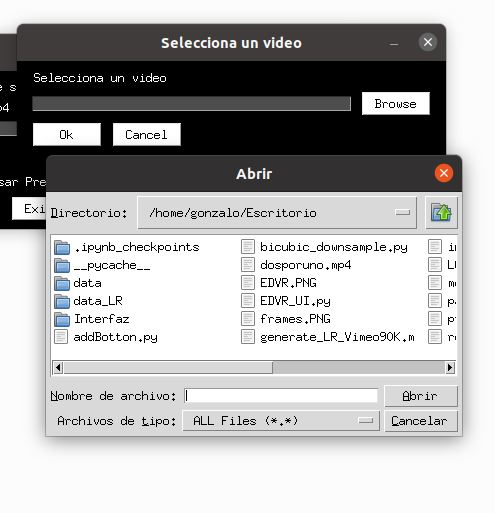
\includegraphics[width=0.8\textwidth]{2}
		\caption{Explorador de archivos para seleccionar el vídeo si no se sabe el \emph{path}}\label{explo}
	\end{figure}

   
   Cuando se hace clic en comenzar, salta una nueva pantalla, se hace clic en generar y empieza la ejecución, el primer paso consiste en convertir el vídeo a fotogramas, cuando la tarea se completa, tardando más cuanto más largo sea el vídeo, salta a la siguiente actualizando el texto y el progreso. 
   
    \imagen{f5}{Barra de referencia para informar de por que parte del procesamiento del vídeo se halla el usuario}
   
   El apartado que más tiempo tarda es el procesado por EDVR, que depende tanto de la duración del vídeo como de la potencia de la máquina que lo esté ejecutando.

    Una vez que acaba todo el proceso se añade un botón y una pregunta que indica si se quiere reproducir el vídeo obtenido mediante el procesamiento.

    \imagen{4}{Reproductor de vídeo}
    
    
\section{Ejemplos de ejecuciones} 

A continuación, se mostrarán algunos ejemplos tanto de vídeos propios procesados por EDVR y ejemplos de los \emph{datasets} usados para el NTIRE Challenge.

  \imagen{pelotaProce}{Primer vídeo propio procesado por EDVR, se observa una pelota cayendo, la imagen de la derecha es la procesada por EDVR.(Imagen adquirida por el autor) }
  
Como se puede observar en la Figura \ref{fig:pelotaProce}, la resolución es mucho mayor, y la calidad es buena. También es muy reseñable la eliminación de las líneas de movimiento alrededor de la pelota.

\imagen{noDedof}{Vídeo en el que se muestra el gesto de negación con el dedo, la imagen de la derecha es la procesada por EDVR. }

En la Figura \ref{fig:noDedof}, las imágenes han sido ampliadas. Como observación general se observa que la imagen izquierda está más pixelada y con menos detalles. En la apliación se muestra el detalle del dedo en movimiento, en la izquierda se observan borrones de movimiento, y en la derecha EDVR ha reconstruido la imagen disminuyendo el emborronamiento, el dedo sigue siendo un poco más grande de lo normal, pero mejora la identificación de la forma básica de un dedo.

Este resultado es muy importante ya que ejemplifica uno de los objetivos del proyecto, ya que aumenta la mejora potencial de la tasa de acierto de métodos automáticos de reconocimiento de gestos y acciones.

\imagen{siCabezaf}{Vídeo en el que se muestra el gesto de afirmación con la cabeza, la imagen de la derecha es la procesada por EDVR.}

La Figura \ref{fig:siCabezaf} muestra el ejemplo de un caso en el que el resultado obtenido no es del todo bueno, en el recuadro de la cara se observa que EDVR no ha procesado bien los movimientos verticales de la cabeza, en la fase de fusionado de imágenes. Pero en contraposición el recuadro de abajo con el dibujo de la camiseta si que se observa bastante mejoría.

\imagen{salto}{Vídeo en el que se muestra el un salto, la imagen de la derecha es la procesada por EDVR.}
En la Figura \ref{fig:salto} se muestra un gesto complejo, ya que el salto es un conjunto de gestos simples. Se muestra el fotograma en medio del aire, en la imagen de la derecha se puede observar mayor calidad con el mismo zoom, las zapatillas se ven mucho menos pixeladas.

\imagen{saltomal}{Captura del vídeo procesado por EDVR en un salto con el modo predeblur.}

En la Figura \ref{fig:saltomal} aparece el mismo fotograma que en la comparación anterior, como se observa el resultado es malo, ya que la figura esta distorsionada, como se observa en el recuadro rojo con la zapatilla. Esto es resultado de usar el modo predeblur cuando no hay emborronamiento. Por lo recomiendo usar solo este modo cuando el  emborronamiento sea abundante.

\begin{figure}[!h]
		\centering
		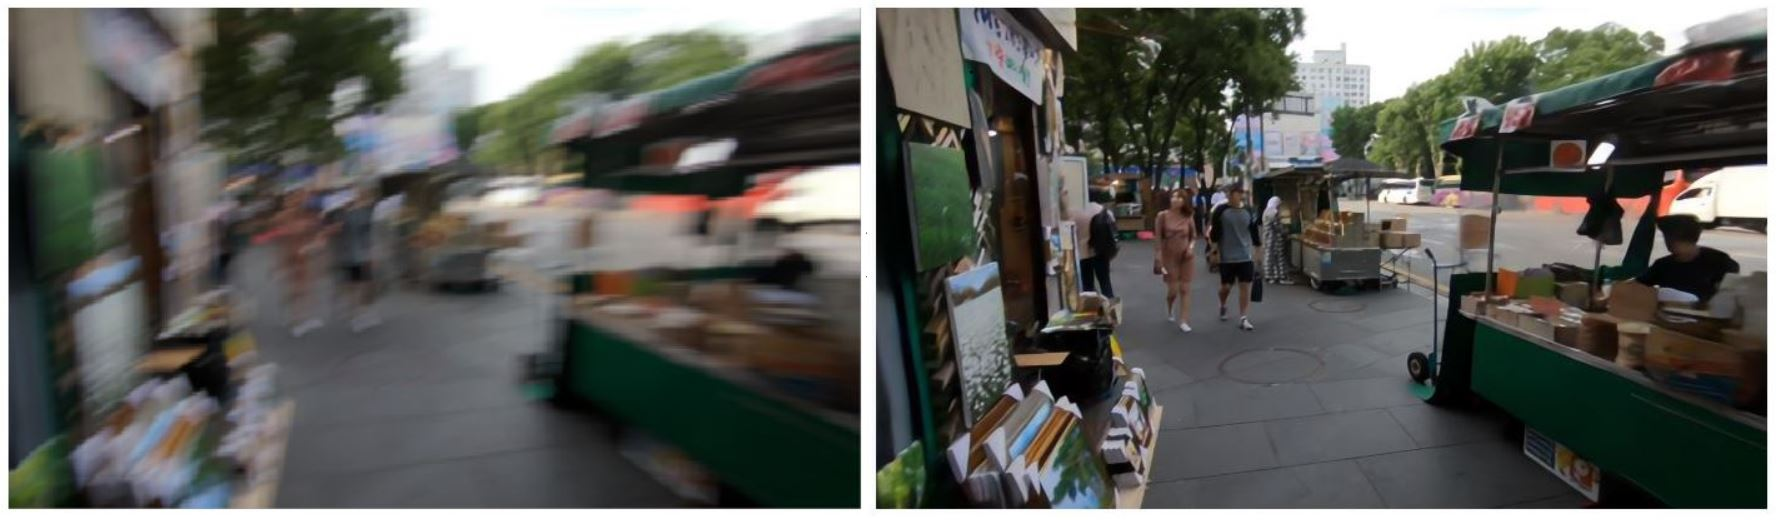
\includegraphics[width=1.1\textwidth]{reds}
		\caption{Vídeo obtenido de REDS, muestra una imagen de un mercado, la imagen de la derecha es la procesada por EDVR~\cite{wang2019edvr}.}\label{5}
	\end{figure}
	\FloatBarrier


Los resultados de la Figura \ref{5} son buenos, lo que muestra la potencia del método en cuanto a su capacidad para mejorar la calidad de los vídeos, también he de decir que el algoritmo está entrenado con imágenes muy parecidas y por eso ofrece mejores resultados que los obtenidos por mí.

\begin{figure}[!h]
		\centering
		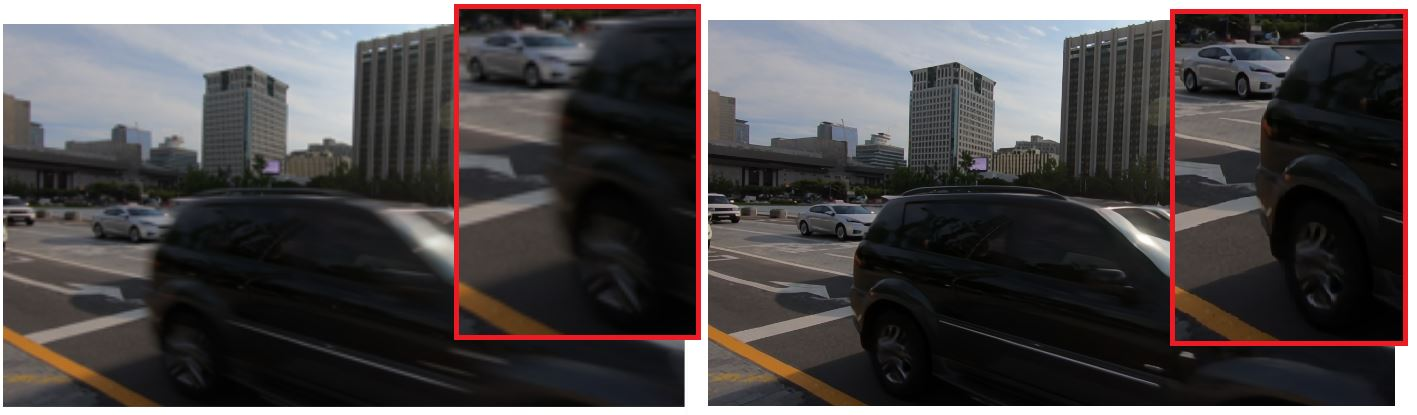
\includegraphics[width=1.1\textwidth]{reds2}
		\caption{Vídeo obtenido de REDS, muestra una imagen de una carretera, la imagen de la derecha es la procesada por EDVR~\cite{wang2019edvr}.}\label{10}
	\end{figure}
	\FloatBarrier

La Figura \ref{10} muestra otra imagen de REDS, esta vez no está tan emborronada, pero también se aprecia muy bien la mejora, solo hay que fijarse en el recuadro rojo que muestra la trasera del coche, como toda la distorsión desaparece y todo está mucho más definido.




